\documentclass{article}
\usepackage[utf8]{inputenc}
\usepackage{polski}
\usepackage{geometry}
\usepackage{pdfpages}
\usepackage{pdfpages}
\usepackage{listings}
\usepackage{listingsutf8}
\usepackage{multirow}
\usepackage{siunitx}
\usepackage{multirow}
\usepackage{booktabs}
\usepackage{tabularx}
\usepackage{placeins}
\usepackage{pdflscape}
\usepackage{graphicx}
\usepackage{subfig}
\usepackage{hyperref}
\usepackage{amsmath}
\usepackage{colortbl}

\geometry{
a4paper,
total={170mm,257mm},
left=20mm,
top=20mm
}
\newcolumntype{Y}{>{\centering\arraybackslash}X}
\renewcommand\thesection{}
\lstset{%
literate=%
 {ą}{{\k{a}}}1
 {ę}{{\k{e}}}1
 {Ą}{{\k{A}}}1
 {Ę}{{\k{E}}}1
 {ś}{{\'{s}}}1
 {Ś}{{\'{S}}}1
 {ź}{{\'{z}}}1
 {Ź}{{\'{Z}}}1
 {ń}{{\'{n}}}1
 {Ń}{{\'{N}}}1
 {ć}{{\'{c}}}1
 {Ć}{{\'{C}}}1
 {ó}{{\'{o}}}1
 {Ó}{{\'{O}}}1
 {ż}{{\.{z}}}1
 {Ż}{{\.{Z}}}1
 {ł}{{\l{}}}1
 {Ł}{{\l{}}}1
}

\title{Metody Obliczeniowe w Nauce i Technice\\ 
Laboratorium I}
\author{Maciej Trątnowiecki}
\date{AGH, Semestr Letni, 2020}

\begin{document}
    \maketitle
    \section{Sumowanie liczb pojedynczej precyzji}
        W ramach laboratorium zaimplementowałem trzy algorytmy obliczające sumę $N$ liczb z tablicy, każdej o wartości $v$. Za $N$ przyjąłem $10^7$, za $v$ początkowo $v=0.53125$. \\
        Obliczyłem błąd względny i bezwzględny jakim obarczone były przeprowadzone operacje arytmetyczne, uzyskując poniższe wyniki. 
        \begin{center}
            \begin{table}[ht]
                \centering
                \begin{tabular}{|c|c|c|c|}
                    \hline
                    Mierzona wartość & Sumowanie proste & Sumowanie rekursywne & Sumowanie Kahana\\
                    \specialrule{1pt}{1pt}{1pt}
                    Wynik sumowania &  5030840.50 & 5312500.00 & 5312500.00\\
                    \hline
                    Błąd bezwzględny & 281659.50 & 0.00 & 0.00\\
                    \hline
                    Błąd względny & 5.30\% & 0.00\% & 0.00\%\\
                    \hline 
                \end{tabular}
                \caption{Wyniki obliczeń dla $v=0.53125$}
                \label{tab:my_label}
            \end{table}
        \end{center}
        Następnie zmieniłem wartość $v$ na $0.63211$, uzyskując poniższe wyniki. 
        \begin{center}
            \begin{table}[ht]
                \centering
                \begin{tabular}{|c|c|c|c|}
                    \hline
                    Mierzona wartość & Sumowanie proste & Sumowanie rekursywne & Sumowanie Kahana\\
                    \specialrule{1pt}{1pt}{1pt}
                    Wynik sumowania &  6119759.50 & 6321100.00 & 6321100.00\\
                    \hline
                    Błąd bezwzględny & 201340.50 & 0.00 & 0.00\\
                    \hline
                    Błąd względny & 3.18\% & 0.00\% & 0.00\%\\
                    \hline 
                \end{tabular}
                \caption{Wyniki obliczeń dla $v=0.63211$}
                \label{tab:my_label}
            \end{table}
        \end{center}
        Błąd względny w algorytmie prostym znacznie rośnie, ponieważ wielokrotnie sumuje on liczby zupełnie różnych rzędów wielkości. Błąd względny jest znacznie mniejszy w algorytmie Kahana, jak i sumowania rekursywnego względem algorytmu prostego. W algorytmie rekursywnym, błąd nie występuje, ponieważ sumowane liczby są tego samego rzędu. Algorytm Kahana śledzi występujący błąd obliczeń i minimalizuje go w kolejnych sumowaniach. Jest to możliwe, ponieważ w zmiennej err przechowywany jest występujący na mniej znaczących bitach błąd dokładności. Żeby go obliczyć, algorytm najpierw oblicza różnicę stosunkowo dużych liczb reprezentujących aktualną i poprzednią sumę, dopiero następnie odejmuje od niego stosunkowo małą dodawaną aktualnie wartość. \\ 
        Prześledziłem również jak wyglądał wzrost błędu w algorytmie prostego sumowania. Zebrane wyniki przedstawiłem na poniższych wykresach. Błękitnymi kropkami oznaczono każdy milion kroków. 
        \begin{figure}[h!]
            \centering
            \subfloat[$v=0.53125$]{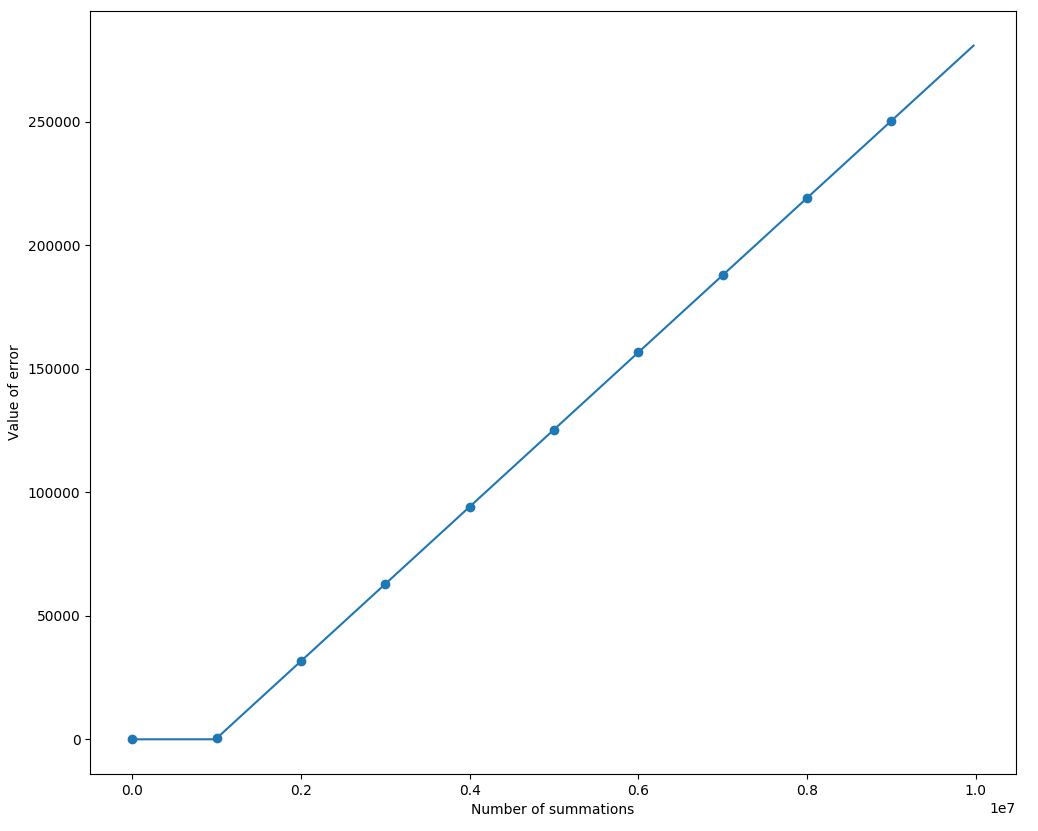
\includegraphics[width=9cm]{lab1/img/ErrorsPlot_1.png}}
            \subfloat[$v=0.63211$]{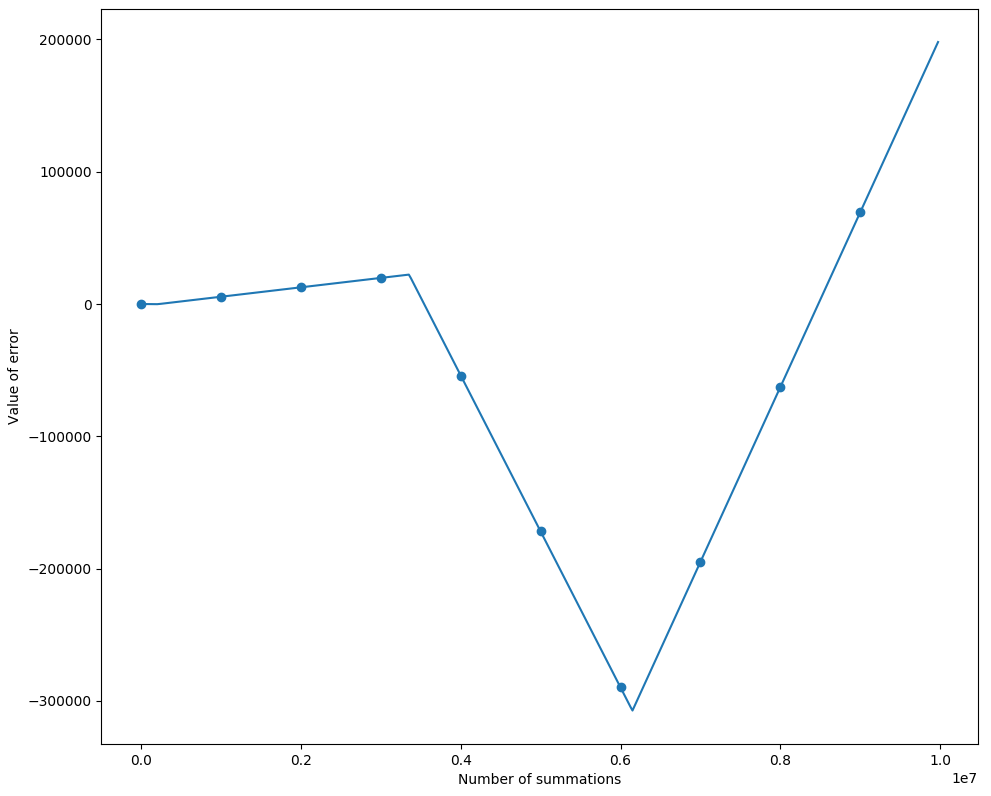
\includegraphics[width=9cm]{lab1/img/ErrorsPlot_2.png}}
            \caption{Wykres zmiany błędu bezwzględnego w stosunku do liczby sumowań.}
        \end{figure}\\
        Łatwo zauważyć, że wykres narastania błędu jest ciągłą sumą funkcji liniowych. W początkowej fazie, gdy dodawane wartości są tego samego rzędu, błąd nie rośnie w ogóle, lub rośnie wolno. 
        \FloatBarrier
        Wykonałem także porównanie czasów wykonania dla każdego z trzech algorytmów. Do pomiarów czasu w sposób powtarzalny użyłem pakietu sio2jail (\url{https://github.com/sio2project/sio2jail}), którego specyfika została lepiej opisana w pracy licencjackiej (\url{https://hitagi.dasie.mimuw.edu.pl/files/licencjat/pracalic-logo.pdf}), za pośrednictwem skryptu opakowującego oiejq (\url{https://oi.edu.pl/static/attachment/20181007/oiejq.tar.gz}), używanego przez Ogólnopolską Olimpiadę Informatyczną. Otrzymałem następujące wyniki.\\
        \begin{center}
            \begin{table}[ht]
                \centering
                \begin{tabular}{|c|c|}
                    \hline
                    Algorytm  & Czas wykonania \\
                    \specialrule{1pt}{1pt}{1pt}
                    Prosty & $21ms$ \\
                    \hline
                    Rekursywny & $156ms$ \\
                    \hline
                    Kahana & $21ms$ \\
                    \hline 
                \end{tabular}
                \caption{Pomiar czasów wykonania}
                \label{tab:my_label}
            \end{table}
        \end{center}\\
        Dla uprzednio rozważanych wartości $v$ zarówno algorytm rekursywny, jak i algorytm Kahana zwracał dokładny wynik. Jednak dla $v=0.666666$ w wyniku działania algorytmu rekursywnego otrzymałem wynik obarczony błędem bezwzględnym rzędu $0.50$, podczas gdy algorytm Kahana zwrócił wynik dokładny. 
        
    \section{Sumy częściowe}    
        Obliczyłem wartość funkcji $\dzeta$ i $\eta$ dla wskazanych parametrów w przód i wstecz. Dla $n< 200$ nie zauważyłem rozbieżności. Otrzymane wyniki zebrałem w poniższej tabeli. Występujące różnice oznaczyłem kolorem pomarańczowym. 
        \begin{center}
            \begin{table}[ht]
                \centering
                \begin{tabular}{|c|c|c|c|c|}
                    \hline
                    Wartość s & $\zeta$ w przód & $\zeta$ wstecz & $\eta$ w przód & $\eta$ wstecz  \\
                    \specialrule{1pt}{1pt}{1pt}
                    $2.0$ & 1.625133 & 1.625133 & 0.822271 & 0.822271 \\
                    \hline
                    $3.6667$ &\cellcolor{orange!40} 1.109399 &\cellcolor{green!40}1.109400  &0.934693  & 0.934693 \\
                    \hline
                    $5.0$ &\cellcolor{orange!40} 1.036927 &\cellcolor{green!40} 1.036928 &  0.972120&  0.972120 \\
                    \hline 
                    $7.2$ & 1.007228 &1.007228  & 0.993527 &  0.993527\\  
                    \hline 
                    $10.0$ & 1.000995 & 1.000995 & 0.999040 & 0.999040 \\
                    \hline 
                \end{tabular}
                \caption{$n=50$, float}
                \label{tab:my_label}
            \end{table}
        \end{center}
        \begin{center}
            \begin{table}[ht]
                \centering
                \begin{tabular}{|c|c|c|c|c|}
                    \hline
                    Wartość s & $\zeta$ w przód & $\zeta$ wstecz & $\eta$ w przód & $\eta$ wstecz  \\
                    \specialrule{1pt}{1pt}{1pt}
                    $2.0$ & 1.634984 &1.634984  & 0.822417 & 0.822417 \\
                    \hline
                    $3.6667$ & 1.109409 & 1.109409 &0.934693  & 0.934693 \\
                    \hline
                    $5.0$ &\cellcolor{orange!40} 1.036927 &\cellcolor{green!40} 1.036928 &0.972120  & 0.972120  \\
                    \hline 
                    $7.2$ & 1.007228 & 1.007228 & 0.993527 & 0.993527 \\  
                    \hline 
                    $10.0$ &1.000995  & 1.000995 &0.999040  & 0.999040 \\
                    \hline 
                \end{tabular}
                \caption{$n=100$, float}
                \begin{tabular}{|c|c|c|c|c|}
                    \hline
                    Wartość s & $\zeta$ w przód & $\zeta$ wstecz & $\eta$ w przód & $\eta$ wstecz  \\
                    \specialrule{1pt}{1pt}{1pt}
                    $2.0$ &\cellcolor{green!40}1.639947  &\cellcolor{orange!40} 1.639946 & 0.822455 & 0.822455 \\
                    \hline
                    $3.6667$ &\cellcolor{orange!40} 1.109409 &\cellcolor{green!40}1.109410  & 0.934693 & 0.934693 \\
                    \hline
                    $5.0$ & \cellcolor{orange!40} 1.036927& \cellcolor{green!40} 1.036928& 0.972120 &  0.972120 \\
                    \hline 
                    $7.2$ &1.007228  & 1.007228 & 0.993527 &  0.993527\\  
                    \hline 
                    $10.0$ & 1.000995 & 1.000995 & 0.999040 & 0.999040 \\
                    \hline 
                \end{tabular}
                \caption{$n=200$, float}
                
                \begin{tabular}{|c|c|c|c|c|}
                    \hline
                    Wartość s & $\zeta$ w przód & $\zeta$ wstecz & $\eta$ w przód & $\eta$ wstecz  \\
                    \specialrule{1pt}{1pt}{1pt}
                    $2.0$ & 1.642936 &  1.642936& 0.822465 & 0.822465 \\
                    \hline
                    $3.6667$ & \cellcolor{orange!40}1.109409 & \cellcolor{orange!40} 1.109411&  0.934693&  0.934693\\
                    \hline
                    $5.0$ & \cellcolor{orange!40}1.036927 &\cellcolor{green!40} 1.036928 & 0.972120 &  0.972120 \\
                    \hline 
                    $7.2$ &  1.007228&  1.007228&  0.993527& 0.993527 \\  
                    \hline 
                    $10.0$ & 1.000995 & 1.000995 &  0.999040& 0.999040 \\
                    \hline 
                \end{tabular}
                \caption{$n=500$, float}
                
                \begin{tabular}{|c|c|c|c|c|}
                    \hline
                    Wartość s & $\zeta$ w przód & $\zeta$ wstecz & $\eta$ w przód & $\eta$ wstecz  \\
                    \specialrule{1pt}{1pt}{1pt}
                    $2.0$ &\cellcolor{green!40} 1.643935 & \cellcolor{orange!40}1.643934 & 0.822467 & 0.822467 \\
                    \hline
                    $3.6667$ & \cellcolor{orange!40} 1.109409&\cellcolor{green!40} 1.109411 & 0.934693 &  0.934693\\
                    \hline
                    $5.0$ & \cellcolor{orange!40} 1.036927&\cellcolor{green!40}  1.036928&  0.972120&   0.972120\\
                    \hline 
                    $7.2$ & 1.007228 & 1.007228 & 0.993527 & 0.993527 \\  
                    \hline 
                    $10.0$ & 1.000995 & 1.000995 & 0.999040 & 0.999040 \\
                    \hline 
                \end{tabular}
                \caption{$n=1000$, float}
                \label{tab:my_label}
            \end{table}
        \end{center}
        \FloatBarrier
        Następnie wykonałem te same obliczenia stosując zmienne zmiennoprzecinkowe podwójnej precyzji, otrzymując te same wyniki licząc w przód i wstecz, dla obu rozpatrywanych funkcji. W miejscach, gdzie przy zastosowaniu pojedynczej precyzji wystąpiły rozbieżności kolorem zielonym oznaczyłem dokładne wartości.\\ W celu wytłumaczenia zaobserwowanych rozbieżności dla wyniku uzyskiwanego w przód i wstecz dla reprezentacji pojedynczej precyzji rozpatrzmy błąd operacji zmiennoprzecinkowych $\epsilon$ dla obu sposobów prowadzenia obliczeń. 
        $$fl(fl(x+y)+z)=fl((x+y)(1+\epsilon)+z)=((x+y)(1+\epsilon)+z)(1+\epsilon)=(x+x\epsilon+y+y\epsilon+z)(1+\epsilon)$$
        $$fl(fl(x+y)+z)=(x+y+z+\epsilon(x+y))(1+\epsilon)$$
        
        $$fl(x+fl(y+z))=fl(x+(y+z)(1+\epsilon))=(x+(y+z)(1+\epsilon))(1+\epsilon)=(x+y+y\epsilon+z+z\epsilon)(1+\epsilon)$$
        $$fl(x+fl(y+z))=(x+y+z+\epsilon(z+y))(1+\epsilon)$$
        
        Zauważmy, że gdy $|x+y|<|y+z|$ w drugiej równości otrzymujemy większy błąd względny. \\
        Możemy stąd wnioskować, że wartość funkcji obliczanej w przód jest obarczona większym błędem względnym, gdyż w pamięci reprezentujemy większą sumę. Przyjmuje ona postać $\frac{1}{1^s}+\frac{1}{2^s}+\frac{1}{3^s}+\ldots+\frac{1}{n^s}$, gdzie $s>1$. Łatwo zauważyć, że początkowe wyrazy ciągu są co do wartości większe od końcowych, zatem ich suma też jest większa. Nie znaczy to jednak, że przy sumowaniu wstecz nie występuje błąd - stąd nie zawsze otrzymany wynik pokrywa się z obliczeniami dokładnymi uzyskanymi po zastosowaniu podwójnej precyzji. 
        
        
    \section{Błędy zaokrągleń i odwzorowanie logistyczne}
        W celu prześledzenia zbieżności procesu iteracyjnego określonego zadanym odwzorowaniem logistycznym przygotowałem interaktywny wykres wartości kolejnych elementów ciągu dla wartości stałej $r$ z przedziału $[1.0, 4.0]$ i $x_0 = 0.77$. Ze względu na ograniczenia techniczne formatu pdf, wspomniany wykres umieściłem pod poniższym adresem \url{http://users.v-lo.krakow.pl/~maciektr/mownit/lab1_logistic_map.gif}.\\
        Za jego pomocą łatwo wywnioskować, że:
        \begin{itemize}
            \item dla $r\in[1.0,2.0]$ - kolejne elementy ciągu szybko zbiegają do swojej granicy. Możemy prosto wyznaczyć ją sposobem wspomniany poniżej.
            \item dla $r\in[2.0,3.0]$ - ciąg jest zbieżny, ale w początkowej fazie waha się. 
            \item dla $r\in[3.0,3.5]$ - odwzorowanie tworzy oscylator.
            \item dla $r\in[3.5,4.0]$ - otrzymujemy chaotyczne drgania. 
        \end{itemize}
        Załóżmy, że ciąg $x_n$ jest zbieżny. Niech $\lim_{n\to\infty} x_n=g$. Wtedy: 
        $$\lim_{n\to\infty} x_{n+1}=g=\lim_{n\to\infty} rx_n(1-x_n)=rg(1-g)\implies r(1-g)=1 \implies g=\frac{r-1}{r}$$
        Następnie przygotowałem wykres bifurkacyjny dla zadanego odwzorowania. Oryginalny obraz, o rozdzielczości $4000\times 4000$ pikseli umieściłem pod następującym adresem \url{http://users.v-lo.krakow.pl/~maciektr/mownit/lab1_bifurcation.png}.
        \begin{figure}[h!]
            \centering
            \subfloat[$x_0=0.7;r\in(1.0, 4.0)$]{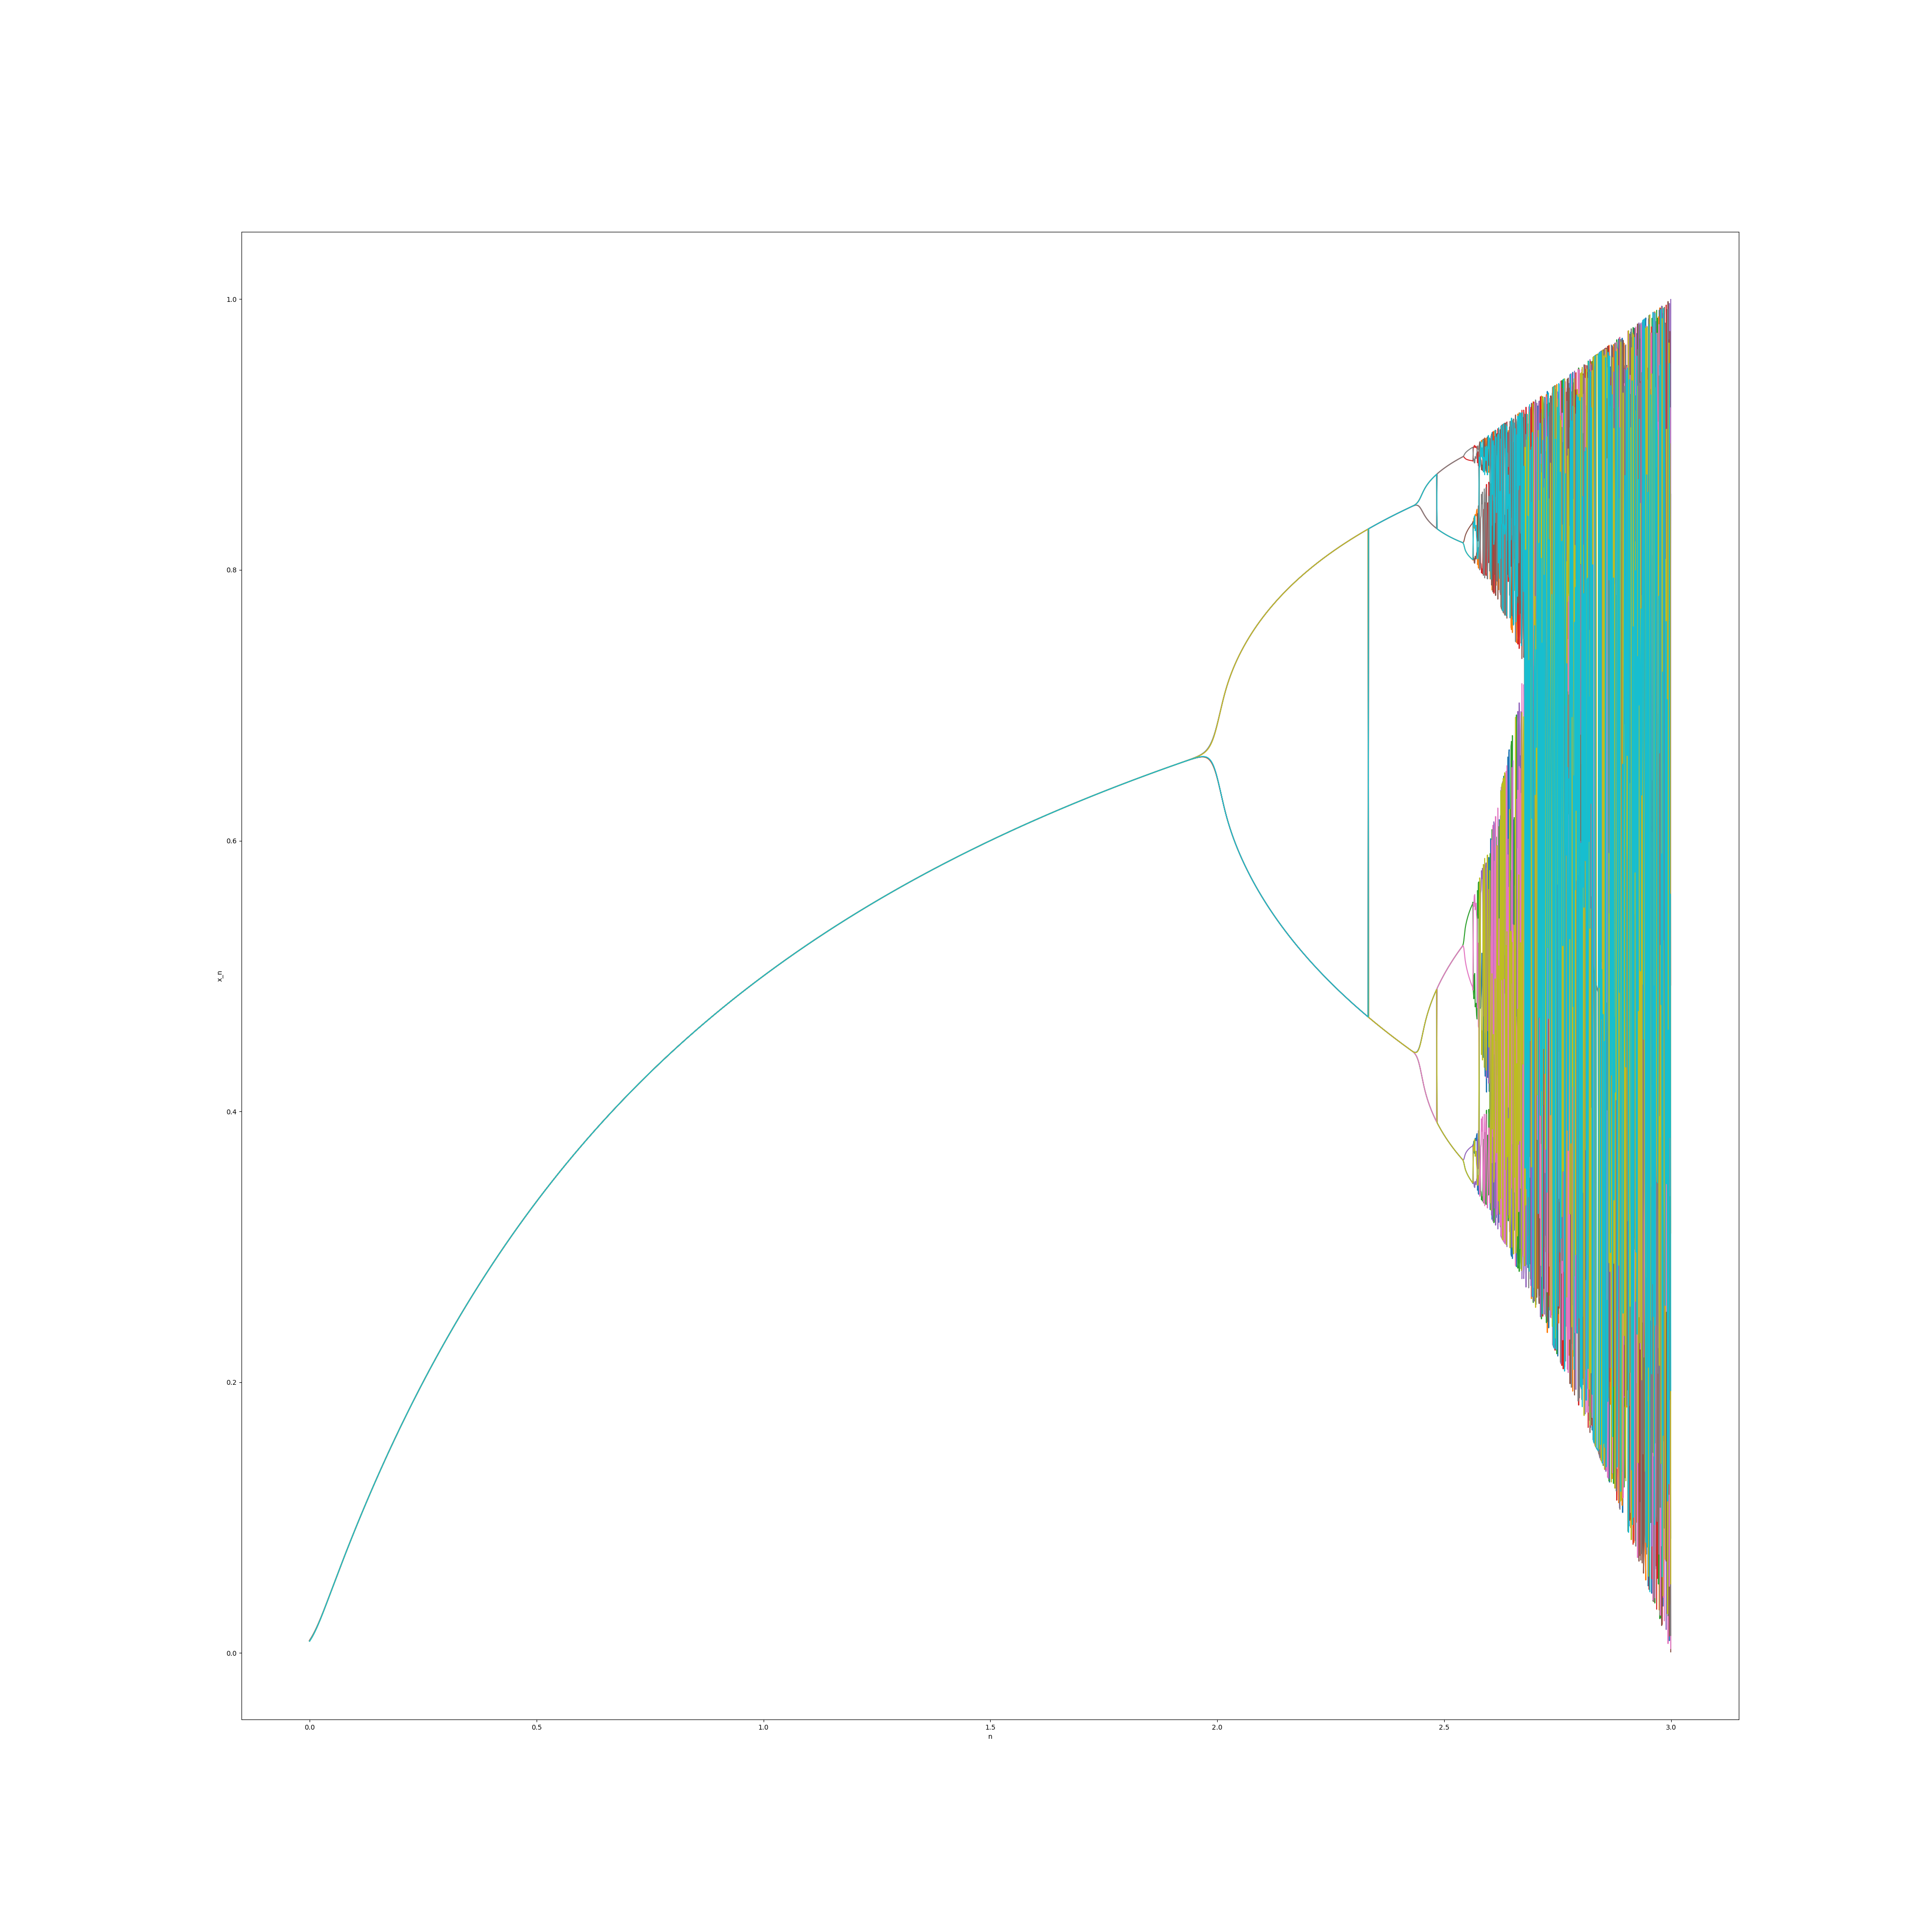
\includegraphics[width=18cm]{lab1/img/Bifurcation_0.png}}
            \caption{Diagram bifurkacyjny.}
        \end{figure}
        \begin{figure}[h!]
            \centering
            \subfloat[$x_0=0.7;r\in(3.5, 4.0)$]{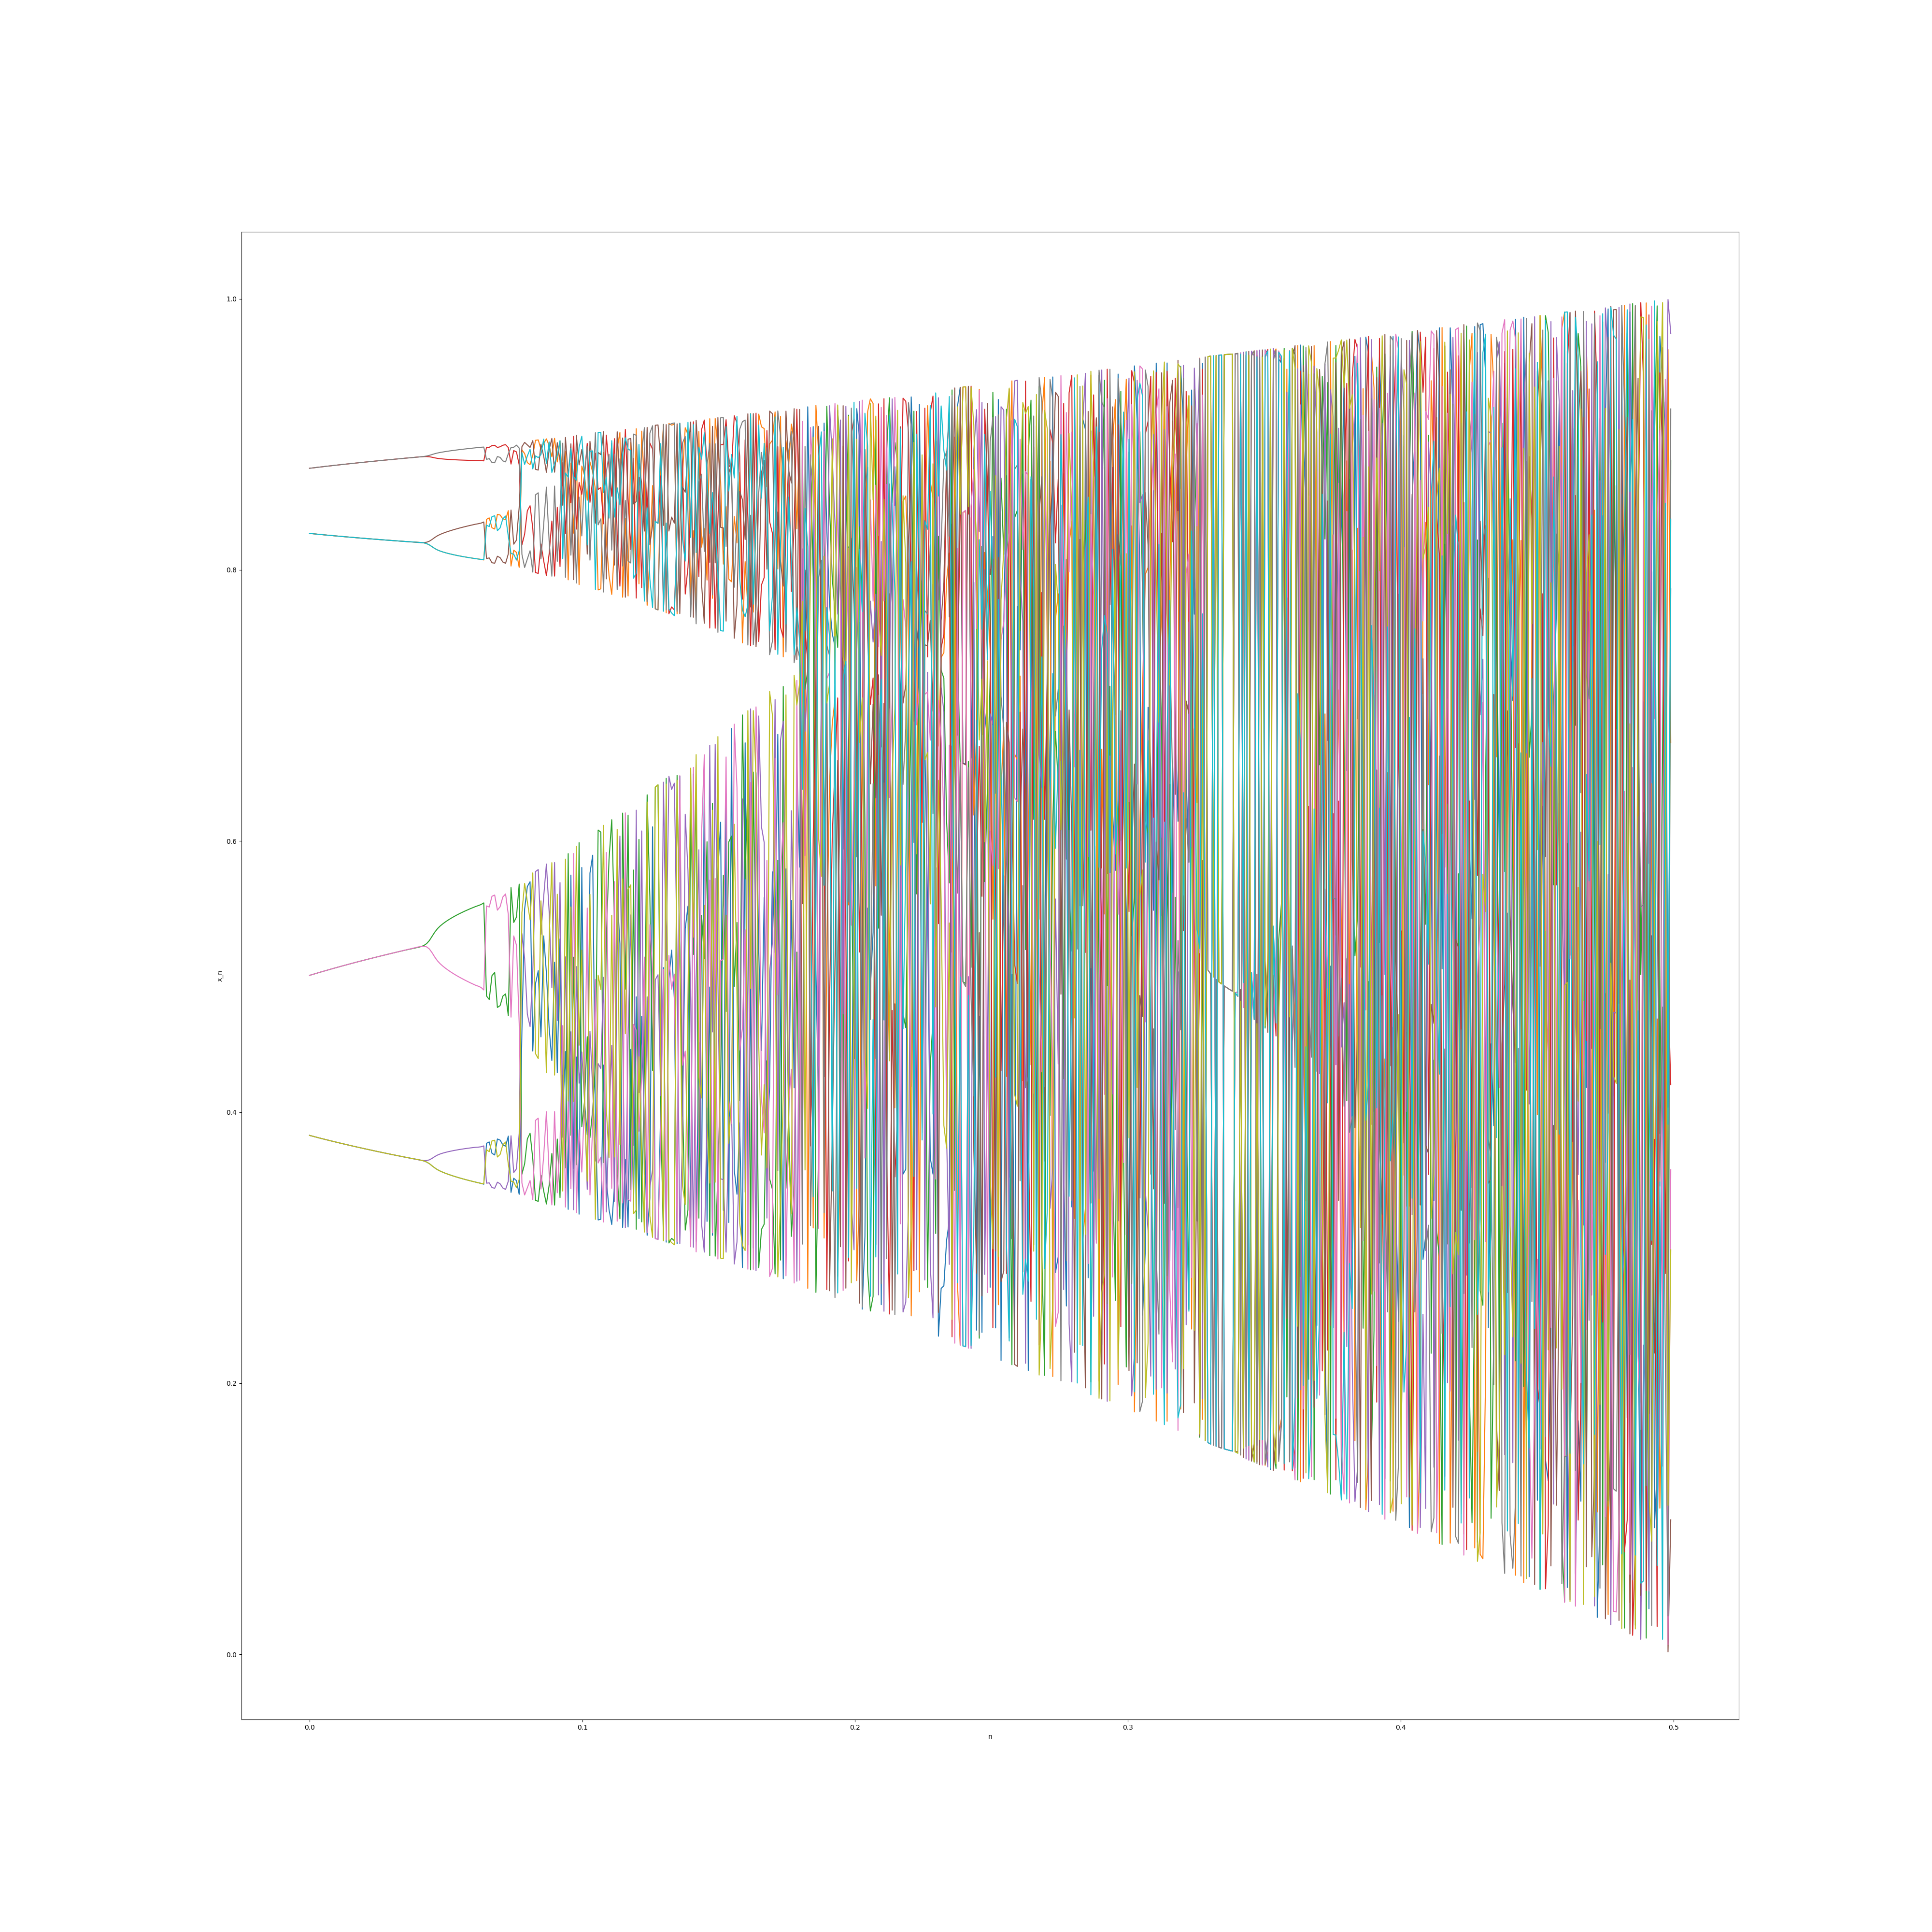
\includegraphics[width=13cm]{lab1/img/Bifurcation_3.png}}\\
            \subfloat[$x_0=0.8;r\in(1.0, 4.0)$]{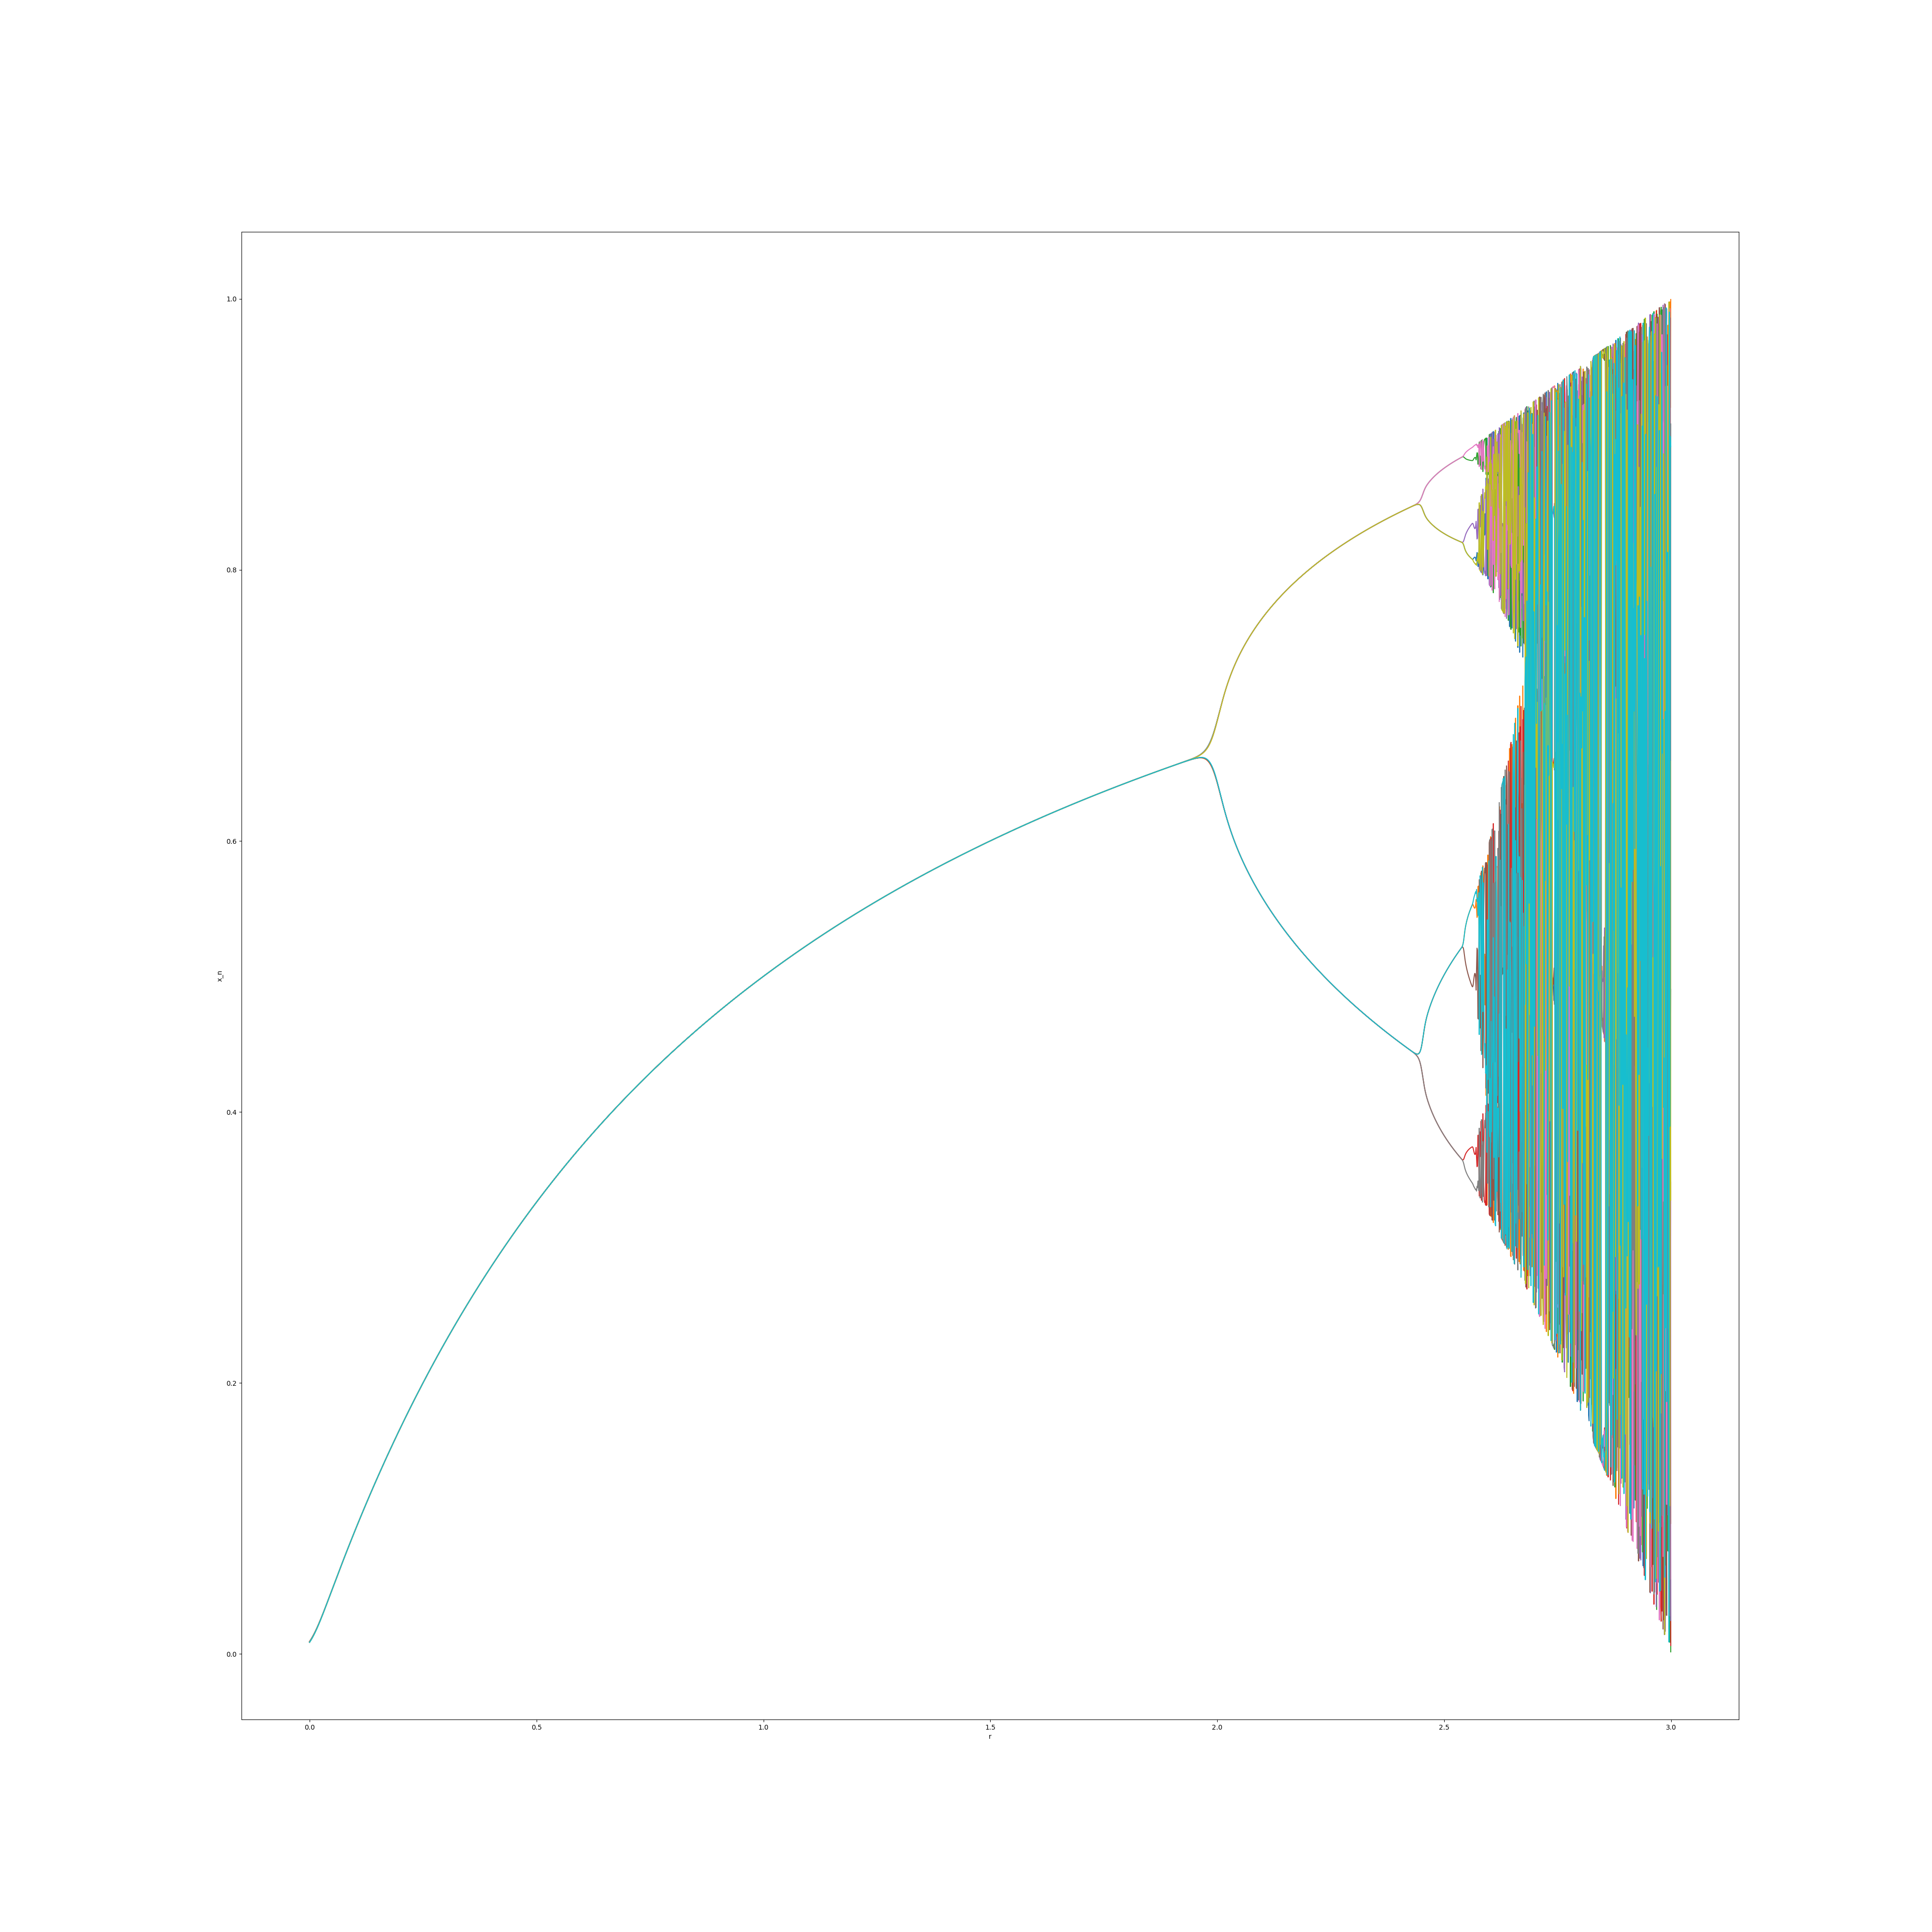
\includegraphics[width=13cm]{lab1/img/Bifurcation_6.png}}
            \caption{Diagram bifurkacyjny.}
        \end{figure}\\
        Diagram bifurkacyjny pokazuje rozwidlanie się stanów stabilnych odwzorowania logistycznego. Widzimy, że oscylacje odbywają się wokół kolejno jednej, dwóch, czterech itd. wartości, aż nie przejdą w chaos. Łatwo zauważyć związek otrzymanego wykresu, z wcześniej określonymi przedziałami zbieżności. 
        \FloatBarrier
        Prześledziłem również zmianę trajektorii liczonych z użyciem pojedynczej i podwójnej precyzji, dla $x_0=0.7$. 
        \begin{figure}[h!]
            \centering
            \subfloat[$r=3.75$, float]{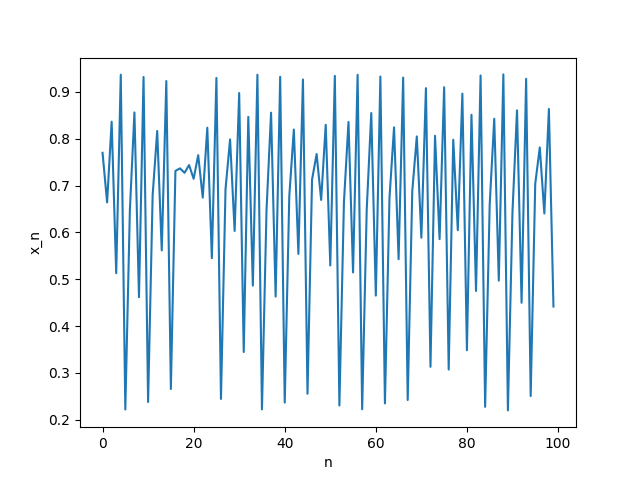
\includegraphics[width=9cm]{lab1/img/trajectory0_float.png}}
            \subfloat[$r=3.75$, double]{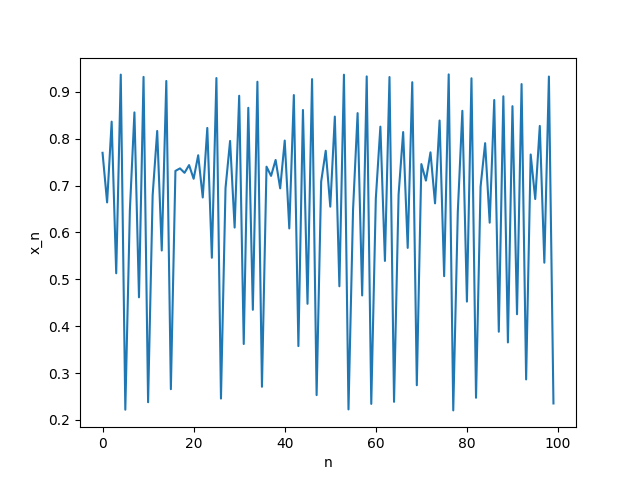
\includegraphics[width=9cm]{lab1/img/trajectory0_double.png}}\\
            \subfloat[$r=3.76$, float]{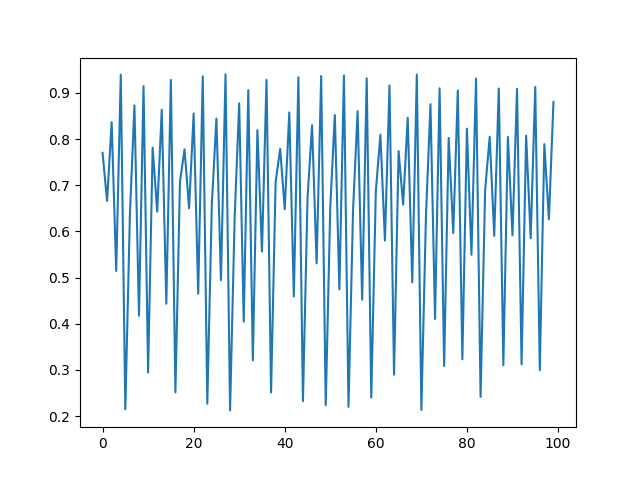
\includegraphics[width=9cm]{lab1/img/trajectory1_float.png}}
            \subfloat[$r=3.76$, double]{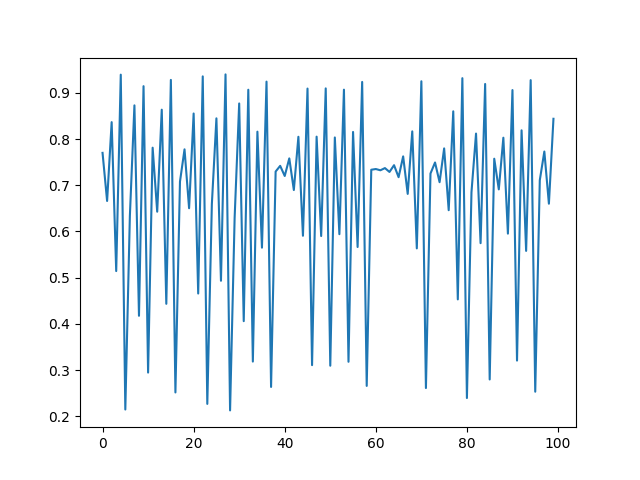
\includegraphics[width=9cm]{lab1/img/trajectory1_double.png}}\\
            \subfloat[$r=3.77$, float]{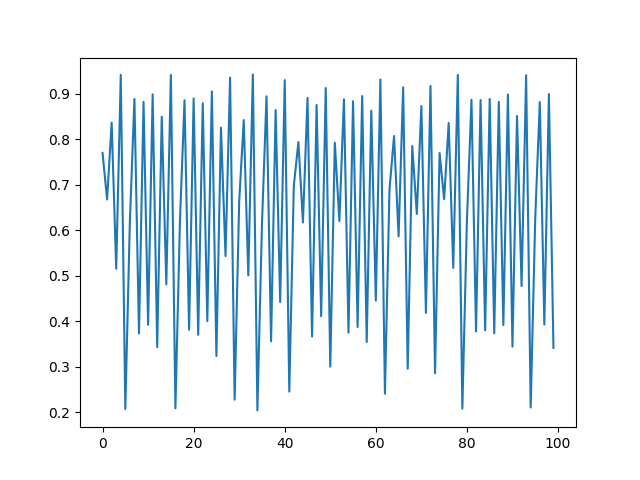
\includegraphics[width=9cm]{lab1/img/trajectory2_float.png}}
            \subfloat[$r=3.77$, double]{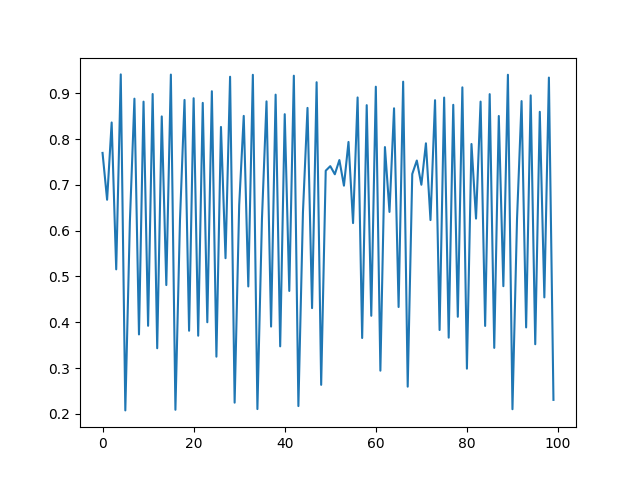
\includegraphics[width=9cm]{lab1/img/trajectory2_double.png}}\\

            \caption{Trajektorie w pojedynczej i podwójnej precyzji.}
        \end{figure}\\
        \begin{figure}[h!]
            \centering        
            \subfloat[$r=3.78$, float]{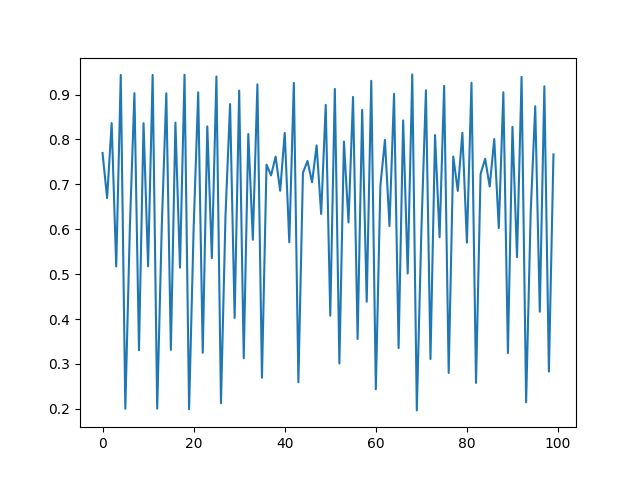
\includegraphics[width=9cm]{lab1/img/trajectory3_float.png}}
            \subfloat[$r=3.78$, double]{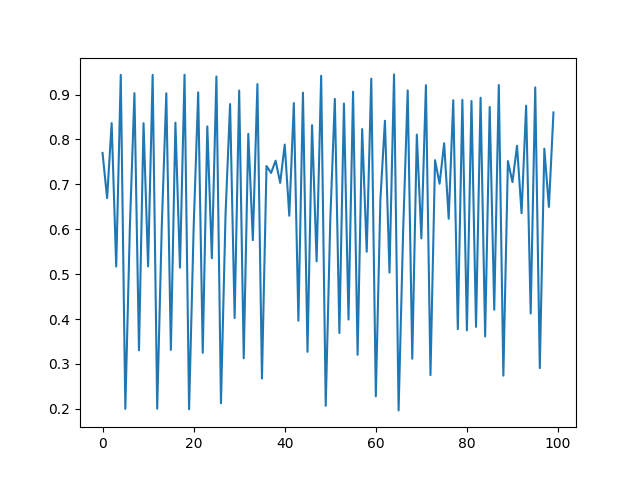
\includegraphics[width=9cm]{lab1/img/trajectory3_double.png}}\\
            \caption{Trajektorie w pojedynczej i podwójnej precyzji.}
        \end{figure}      
        \FloatBarrier
        Widzimy, że użycie podwójnej precyzji obliczeń skutkuje otrzymaniem zmienionej trajektorii w porównaniu z pojedynczą precyzją, jednak dalej ma ona charakter chaotyczny.\\ 
        
        Następnie wyznaczyłem liczbę iteracji potrzebnych do osiągnięcia zera w pojedynczej precyzji, dla $r = 4$.\\
        Dla $x_0=0.77$, otrzymałem $4135$ iteracji, przyjmując dokładność $\epsilon = 4.8*10^{-7}$.\\ Dla $x_0=0.6$ otrzymałem $400$ iteracji, z tą samą dokładnością.\\ Dla $v=0.8$ otrzymałem $757$ iteracji z dokładnością $\epsilon = 5.5*10^{-6}$.\\ Porównując z zerem liczby zmiennoprzecinkowe pojedynczej precyzji musimy godzić się na przyjęcie dokładności porównania. W innym wypadku nie otrzymamy poprawnego wyniku. Największa dokładność z jaką możemy dokonać porównania zależna jest od danych wejściowych. 
\end{document}